% Chapter Template

\chapter{Programs and Results} % Main chapter title

\label{Chapter 2} % Change X to a consecutive number; for referencing this chapter elsewhere, use \ref{ChapterX}

%----------------------------------------------------------------------------------------
%	SECTION 1
%----------------------------------------------------------------------------------------

\section{Calculating Pi }
To calculate the value of $\pi$ we decided to utilize the Monte Carlo method. The algorithm is as follows given that a circle and a square have a ratio of areas that is equal to $\pi$ / 4: 

1. Draw a circle inscribed within a square. ( Figure \ref{fig:Monte-carlo} )\\
2. Randomly pick points within the area of the square.\\
3. Find the ratio of the number of points falling within the circle to the total of number of points.\\
4. The ratio of those points should be $\pi$ / 4.\\
5. To obtain the value of $\pi$ , multiply by 4.\\

The more random points (or "darts") thrown into the given area, the more accurate the value of pi will be. This is because as the numerator (number of points within the circle) and denominator (number of total points) gets larger, there will numbers with more decimal places. The following subsections will discuss the implementation of the above algorithm in three different MPI programming paradigms.

\begin{figure}
\centering
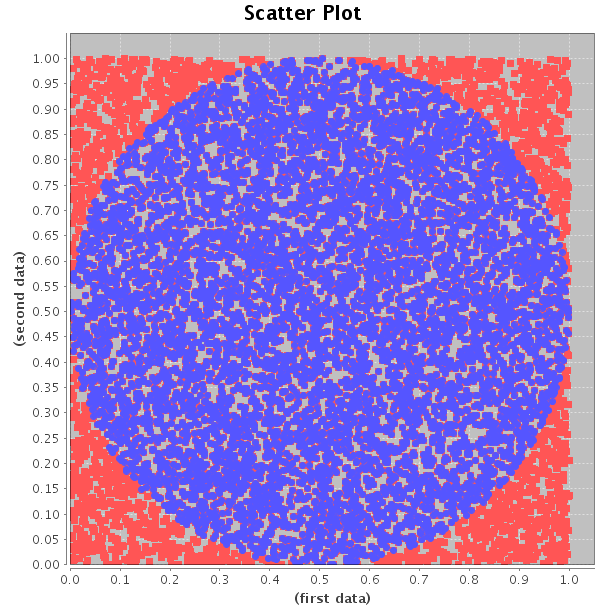
\includegraphics[scale=0.4]{Figures/monte-carlo}
\decoRule
\caption[Monte-Carlo Method]{Depiction of Monte Carlo method to calculate $\pi$ .}
\label{fig:Monte-carlo}
\end{figure}

\subsection {Collective Communication Operations}

One program that we used to calculate $\pi$ utilized the collective communication operations (CCO) method. The collective operation heavily relies on the communicator object which holds necessary information for assigning nodes their respective rank or job number. All processes (or in this case nodes) call the communicator object with the same arguments which ensures synchonization. Note, this is the most primitive form of parallel processing for our purposes as the problem is divided up and the slave  nodes perform the same operations. Susbequently, this is not the most efficient way to program a parallel job as not all job management should be hinged on the actual operation that needs to be completed.


\subsection {Dynamic Process Management}
With the advent of the MPI-2 standard, the implementation of dynamic processes has become much more common place with dynamic process management (DPM). DPM allows parent processes to create new child processes during runtime using spawn functionality. In addition, it can connect previously existing processes with each other with intercommunicator objects. The spawn function can create communicator objects with the original arguments or it can take new arguments.

	Dynamic Process Management (DPA) is used in the master (or parent) process to spawn new worker (or child) processes running a Python interpreter. The master process uses a separate thread to communicate back and forth with the workers. The worker processes serve the execution of tasks in the main (and only) thread until they are signaled for completion. DPA can be really useful in our RPi cluster, because the process model provides a mechanism to create new processes and establish communication between them and the existing MPI application. It also provides mechanisms to establish communication between two existing MPI applications, even when one did not start the other.

	Although DPM offers much more flexibility and efficiency by handling bottlenecks, it requires much more code in order to implement. The code has to determine what jobs will be done by respective child process and how to handle multi-stage spawning. Multi-stage spawning occurs when two child process have to communicate with each other. The programmer has to determine if the child process will communicate with each other directly or if the parent node will act as the intercommunicator. See Figure \ref{fig:Multi-stage} for a visual representation of the parent job in blue with respective child jobs in green.
	
\begin{figure}
\centering
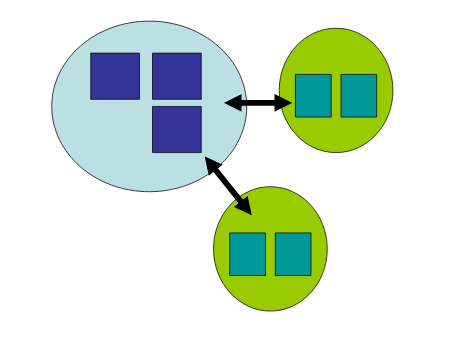
\includegraphics[scale=0.7]{Figures/multi-stage}
\decoRule
\caption[Multi-stage spawning]{An instance of multi-stage spawning.}
\label{fig:Multi-stage}
\end{figure}

\subsection {Remote Memory Access}
Remote memory access (RMA) is another feature implemented in MPI-2. RMA is highly convenient for parallel programming as it does not require the programmer to have send and receive calls for both sides of communication. For instance, all previous programs required an explicit call to send the data and an explicit call to receive the data. The RMA method allows one method call to send the data and at the same time it will automatically initiate a call to receive the data when necessary. This allows processes to act independently of each other when sending and receiving data. Traditionally, when a process sends a job or piece of data to another process or job, it has to wait until that information has been received. With RMA, once the information has been sent, the process is free to move onto its next task. For RMA to work, the process must specify a contiguous region of memory called a window that is open to all other processes. The other processes that are trying to access this space of memory must be aware of this window.

	Remote Memory Access (RMA) supplements the traditional two-sided, send/receive based MPI communication model with a one-sided, put/get based interface. One-sided communication that can take advantage of the capabilities of highly specialized network hardware. Additionally, this extension lowers latency and software overhead in applications written using a shared-memory-like paradigm, which is especially useful in massively parallel computer clusters (in our case our RPi cluster). The MPI specification revolves around the use of objects called windows; they intuitively specify regions of a process’s memory that have been made available for remote read and write operations. The published memory blocks can be accessed through three functions for put (remote send), get (remote write), and accumulate (remote update or reduction) data items. It is useful in calculating pi because in a reduce operation when all processes are sending a value to the original process via RMA it obtains the value of pi much faster.

\section{Results}
During the testing process, we decided to specify four nodes for the parallel processing. The RPi 3 was used as the master node where we executed programs and the RPi Zeros were the slave nodes which executed the specified job. It is important to note that all nodes of the Raspberry Pi require access to the program that is being executed. To solve this problem, we mounted a SSH filesystem (SSHFS) which means that when a file is updated in a directory, that change is made across all systems that have the directory mounted. 

Figure \ref{fig:Results} depicts the time it took to calculate the value of $\pi$ using the three different parallel processing methods. 

\begin{figure}
\centering
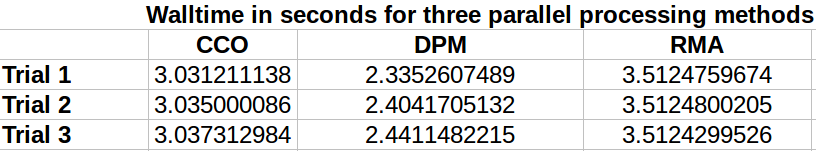
\includegraphics[scale=0.4]{Figures/walltime}
\decoRule
\caption[Results]{Walltime of three different execution methods.}
\label{fig:Results}
\end{figure} 

From the results, we can see that the dynamic process managament (DPM) method had the highest efficiency which may be attributed to its extremely efficienct scheduling system. The collective communications and remote memory methods had very similar execution times. In addition, the DPM method had the lowest error when compared to the actual value of pi. Even more interesting is that the CCO and RMA methods had the same error values which may be attributed to the similar algorithmic implementations of the Monte Carlo Method. 


\begin{figure}
\centering
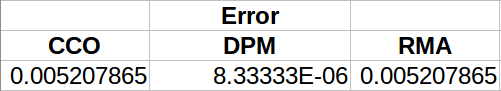
\includegraphics[scale=0.4]{Figures/error}
\decoRule
\caption[Error]{The error between the calcuated and known values of $\pi$}
\label{fig:Error}
\end{figure}